\section*{付録I:電池の種類}

爆弾が使用するタイマーの電池の種類を知ることは、いくつかのセキュリティモジュールを解除する際に非常に重要です。タイマーの電池は通常、タイマーの隣に配置されます。

\begin{center}
\def\arraystretch{1.5}
\begin{tabular}{|>{\centering}p{0.3\textwidth}|p{0.6\textwidth}<{\centering}|}
    \hline
    絵図 & 電池パラメータ \\ \hline
    \parbox[c]{0.3\textwidth}{
        \centering
        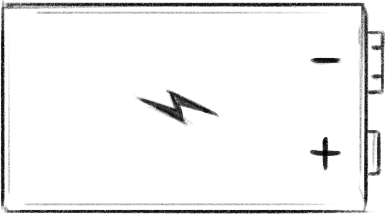
\includegraphics[width=0.25\textwidth]{images/65.png}
    } &
    \parbox[c]{0.6\textwidth}{
        \vspace*{1em}
        種類:6LR61\\
        電圧:9.0 V\\
        セル:二酸化マンガン亜鉛\\
        ホルダー:1つ
        \vspace*{1em}
    }\\ \hline
    \parbox[c]{0.3\textwidth}{
        \centering
        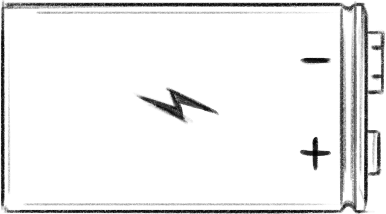
\includegraphics[width=0.25\textwidth]{images/66.png}
    } &
    \parbox[c]{0.6\textwidth}{
        \vspace*{1em}
        種類:6LS05\\
        電圧:9.2 V\\
        セル:二酸化マンガン亜鉛\\
        ホルダー:1つ
        \vspace*{1em}
    }\\ \hline
    \parbox[c]{0.3\textwidth}{
        \centering
        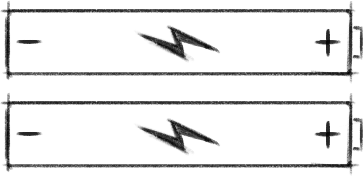
\includegraphics[width=0.25\textwidth]{images/67.png}
    } &
    \parbox[c]{0.6\textwidth}{
        \vspace*{1em}
        種類:CR61\\
        電圧:2 $\times$ 1.3 V\\
        セル:二酸化マンガンリチウム\\
        ホルダー:2つ、同じ方向
        \vspace*{1em}
    }\\ \hline
    \parbox[c]{0.3\textwidth}{
        \centering
        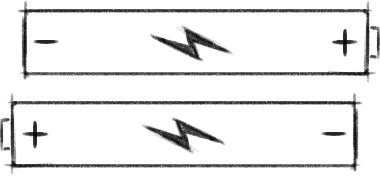
\includegraphics[width=0.25\textwidth]{images/68.png}
    } &
    \parbox[c]{0.6\textwidth}{
        \vspace*{1em}
        種類:CR61\\
        電圧:2 $\times$ 1.3 V\\
        セル:二酸化マンガンリチウム\\
        ホルダー:2つ、反対方向
        \vspace*{1em}
    }\\ \hline
    \parbox[c]{0.3\textwidth}{
        \centering
        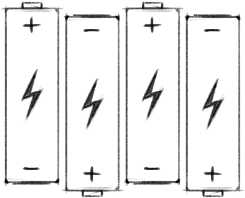
\includegraphics[width=0.25\textwidth]{images/69.png}
    } &
    \parbox[c]{0.6\textwidth}{
        \vspace*{2em}
        種類:2SF11\\
        電圧:4 $\times$ 2.0 V\\
        セル:酸化銀\\
        ホルダー:4つ、反対方向
        \vspace*{2em}
    }\\ \hline
    \parbox[c]{0.3\textwidth}{
        \centering
        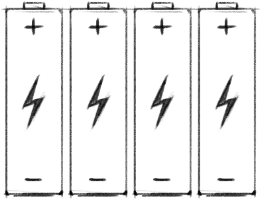
\includegraphics[width=0.25\textwidth]{images/70.png}
    } &
    \parbox[c]{0.6\textwidth}{
        \vspace*{2em}
        種類:2SF11\\
        電圧:4 $\times$ 2.0 V\\
        セル:酸化銀\\
        ホルダー:4つ、同じ方向
        \vspace*{2em}
    }\\ \hline
\end{tabular}
\end{center}

